\documentclass[11pt,english]{article}
\pagestyle{plain}
\pagenumbering{arabic}
\usepackage[english]{babel}
\usepackage{graphicx}
\usepackage{multirow}
\usepackage{subfig}
%\usepackage{auto-pst-pdf}
\usepackage[table,xcdraw]{xcolor}
\usepackage[T1]{fontenc}
\usepackage{hyperref}
\usepackage[hmargin={0.8cm,1.2cm},vmargin=1.2cm]{geometry}
\usepackage{lscape}
\usepackage{pdflscape}
\renewcommand*\familydefault{\sfdefault}
\newcommand{\HRule}{\rule{\linewidth}{0.5mm}}
% packages for headers and footers
\usepackage{fancyhdr}
%\usepackage{lastpage}
\pagestyle{fancy}
\fancyhf{}
%\fancyfoot[C]{Page\ \thepage\ of \pageref{LastPage}}

\begin{document}

\begin{figure}
\begin{center}
\hspace{1.5cm}
\parbox{5.5cm}{
\includegraphics[width=2.2cm]{/home/report/scripts/LOGOS/logoLaMMA}}
\hspace{.3cm}
\parbox{5.5cm}{
\includegraphics[width=2.2cm]{/home/report/scripts/LOGOS/fate_logo_11def}}
\hspace{.3cm}
\parbox{5.5cm}{
\includegraphics[width=2.2cm]{/home/report/scripts/LOGOS/logoINAFBIS}}
\hspace{.1cm}
\vspace{1.2cm}
\end{center}
\end{figure}

\begin{center}
\HRule \\[0.4cm]
%\Huge{\textbf{Progetto FATE LaMMA-OAA per ESO @ Cerro Paranal etcetcetc\ldots}}
\Huge{\textbf{Forecast system for the turbulence and meteorology at the Paranal Observatory}}
\\[0.4cm]
\LARGE{\textbf{Performance assessment - monthly report}}
\HRule \\[0.4cm]
\end{center}

\begin{center}
\vspace{2cm}\Huge{Issued: gio, 04-05-2023\\ 11:48 Paranal local time}
\HRule \\[0.1cm]
\end{center}

%\begin{center}
%\HRule \\[0.1cm]
%\tableofcontents
%\HRule \\[0.1cm]
%\end{center}
%\newpage
\clearpage

%%%%%%%%%%%%%%%%%%%%%%%%%%%%%%%%%
\begin{figure}
\centering
\subfloat[]{\includegraphics[width=.33\linewidth,angle=-90]{/home/report/FIGS/5GG/1H/ws_sim_mnh_ar_dimm_300_960_BEF_stan.eps}}
\subfloat[]{\includegraphics[width=.33\linewidth,angle=-90]{/home/report/FIGS/5GG/1H/ws_sim_mnh_ar_dimm_300_960_AFT_stan.eps}}
\subfloat[]{\includegraphics[width=.33\linewidth,angle=-90]{/home/report/FIGS/5GG/1H/ws_sim_mnh_ar_dimm_300_960_AFT_stan_per.eps}}
\caption{Wind speed ($m s^{-1}$): (a) STANDARD CONFIGURATION, (b) WITH AR, (c) PERSISTENCE.}
\label{fig:ws}
\end{figure}
%%%%%%%%%%%%%%%%%%%%%%%%%%%%%%%%%
\begin{figure}
\centering
\subfloat[]{\includegraphics[width=.33\linewidth,angle=-90]{/home/report/FIGS/5GG/1H/wd_sim_mnh_ar_dimm_300_960_BEF_stan.eps}}
\subfloat[]{\includegraphics[width=.33\linewidth,angle=-90]{/home/report/FIGS/5GG/1H/wd_sim_mnh_ar_dimm_300_960_AFT_stan.eps}}
\subfloat[]{\includegraphics[width=.33\linewidth,angle=-90]{/home/report/FIGS/5GG/1H/wd_sim_mnh_ar_dimm_300_960_AFT_stan_per.eps}}
\caption{Wind direction (degree): (a) STANDARD CONFIGURATION, (b) WITH AR, (c) PERSISTENCE.}
\label{fig:wd}
\end{figure}
%%%%%%%%%%%%%%%%%%%%%%%%%%%%%%%%%
\begin{figure}
\centering
\subfloat[]{\includegraphics[width=.33\linewidth,angle=-90]{/home/report/FIGS/5GG/1H/rh_sim_mnh_ar_dimm_300_960_BEF_stan.eps}}
\subfloat[]{\includegraphics[width=.33\linewidth,angle=-90]{/home/report/FIGS/5GG/1H/rh_sim_mnh_ar_dimm_300_960_AFT_stan.eps}}
\subfloat[]{\includegraphics[width=.33\linewidth,angle=-90]{/home/report/FIGS/5GG/1H/rh_sim_mnh_ar_dimm_300_960_AFT_stan_per.eps}}
\caption{Relative humidity (percent): (a) STANDARD CONFIGURATION, (b) WITH AR, (c) PERSISTENCE.}
\label{fig:rh}
\end{figure}
%%%%%%%%%%%%%%%%%%%%%%%%%%%%%%%%%
\begin{figure}
\centering
\subfloat[]{\includegraphics[width=.33\linewidth,angle=-90]{/home/report/FIGS/5GG/1H/pwv_sim_mnh_ar_dimm_300_960_BEF_stan.eps}}
\subfloat[]{\includegraphics[width=.33\linewidth,angle=-90]{/home/report/FIGS/5GG/1H/pwv_sim_mnh_ar_dimm_300_960_AFT_stan.eps}}
\subfloat[]{\includegraphics[width=.33\linewidth,angle=-90]{/home/report/FIGS/5GG/1H/pwv_sim_mnh_ar_dimm_300_960_AFT_stan_per.eps}}
\caption{Precipitable water vapor (mm): (a) STANDARD CONFIGURATION, (b) WITH AR, (c) PERSISTENCE.}
\label{fig:pwv}
\end{figure}
%%%%%%%%%%%%%%%%%%%%%%%%%%%%%%%%%
\begin{figure}
\centering
\subfloat[]{\includegraphics[width=.33\linewidth,angle=-90]{/home/report/FIGS/5GG/1H/see_sim_mnh_ar_dimm_300_960_BEF_os18_1000.eps}}
\subfloat[]{\includegraphics[width=.33\linewidth,angle=-90]{/home/report/FIGS/5GG/1H/see_sim_mnh_ar_dimm_300_960_AFT_os18_1000.eps}}
\subfloat[]{\includegraphics[width=.33\linewidth,angle=-90]{/home/report/FIGS/5GG/1H/see_sim_mnh_ar_dimm_300_960_AFT_os18_1000_per.eps}}
\caption{Total seeing (arcsec): (a) STANDARD CONFIGURATION, (b) WITH AR, (c) PERSISTENCE.}
\label{fig:see}
\end{figure}
%%%%%%%%%%%%%%%%%%%%%%%%%%%%%%%%%
\begin{figure}
\centering
\subfloat[]{\includegraphics[width=.33\linewidth,angle=-90]{/home/report/FIGS/5GG/1H/tau_sim_mnh_ar_dimm_300_960_BEF_os18_1000.eps}}
\subfloat[]{\includegraphics[width=.33\linewidth,angle=-90]{/home/report/FIGS/5GG/1H/tau_sim_mnh_ar_dimm_300_960_AFT_os18_1000.eps}}
\subfloat[]{\includegraphics[width=.33\linewidth,angle=-90]{/home/report/FIGS/5GG/1H/tau_sim_mnh_ar_dimm_300_960_AFT_os18_1000_per.eps}}
\caption{Coeherence time (ms): (a) STANDARD CONFIGURATION, (b) WITH AR, (c) PERSISTENCE.}
\label{fig:tau}
\end{figure}
%%%%%%%%%%%%%%%%%%%%%%%%%%%%%%%%%
\begin{figure}
\centering
\subfloat[]{\includegraphics[width=.33\linewidth,angle=-90]{/home/report/FIGS/5GG/1H/glf_sim_mnh_ar_dimm_300_960_BEF_os18.eps}}
\subfloat[]{\includegraphics[width=.33\linewidth,angle=-90]{/home/report/FIGS/5GG/1H/glf_sim_mnh_ar_dimm_300_960_AFT_os18.eps}}
\subfloat[]{\includegraphics[width=.33\linewidth,angle=-90]{/home/report/FIGS/5GG/1H/glf_sim_mnh_ar_dimm_300_960_AFT_os18_per.eps}}
\caption{Ground layer fraction (dimensionless): (a) STANDARD CONFIGURATION, (b) WITH AR, (c) PERSISTENCE.}
\label{fig:glf}
\end{figure}
%%%%%%%%%%%%%%%%%%%%%%%%%%%%%%%%%
\begin{figure}
\centering
\subfloat[]{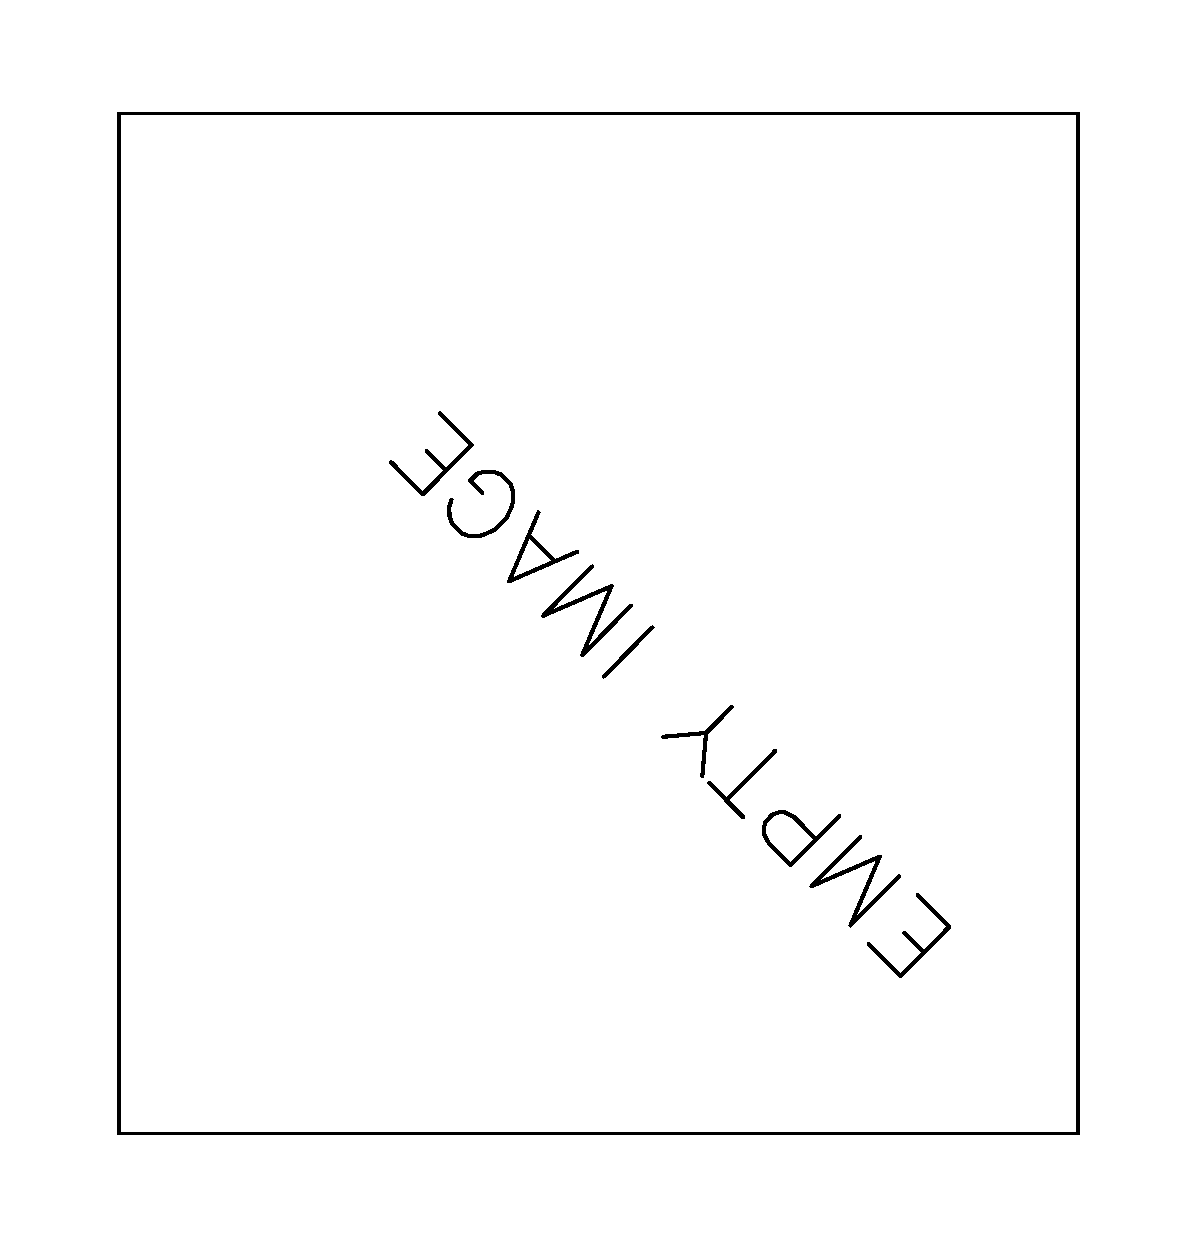
\includegraphics[width=.27\linewidth,angle=-90]{/home/report/FIGS/5GG/1H/emptyimg}}
\subfloat[]{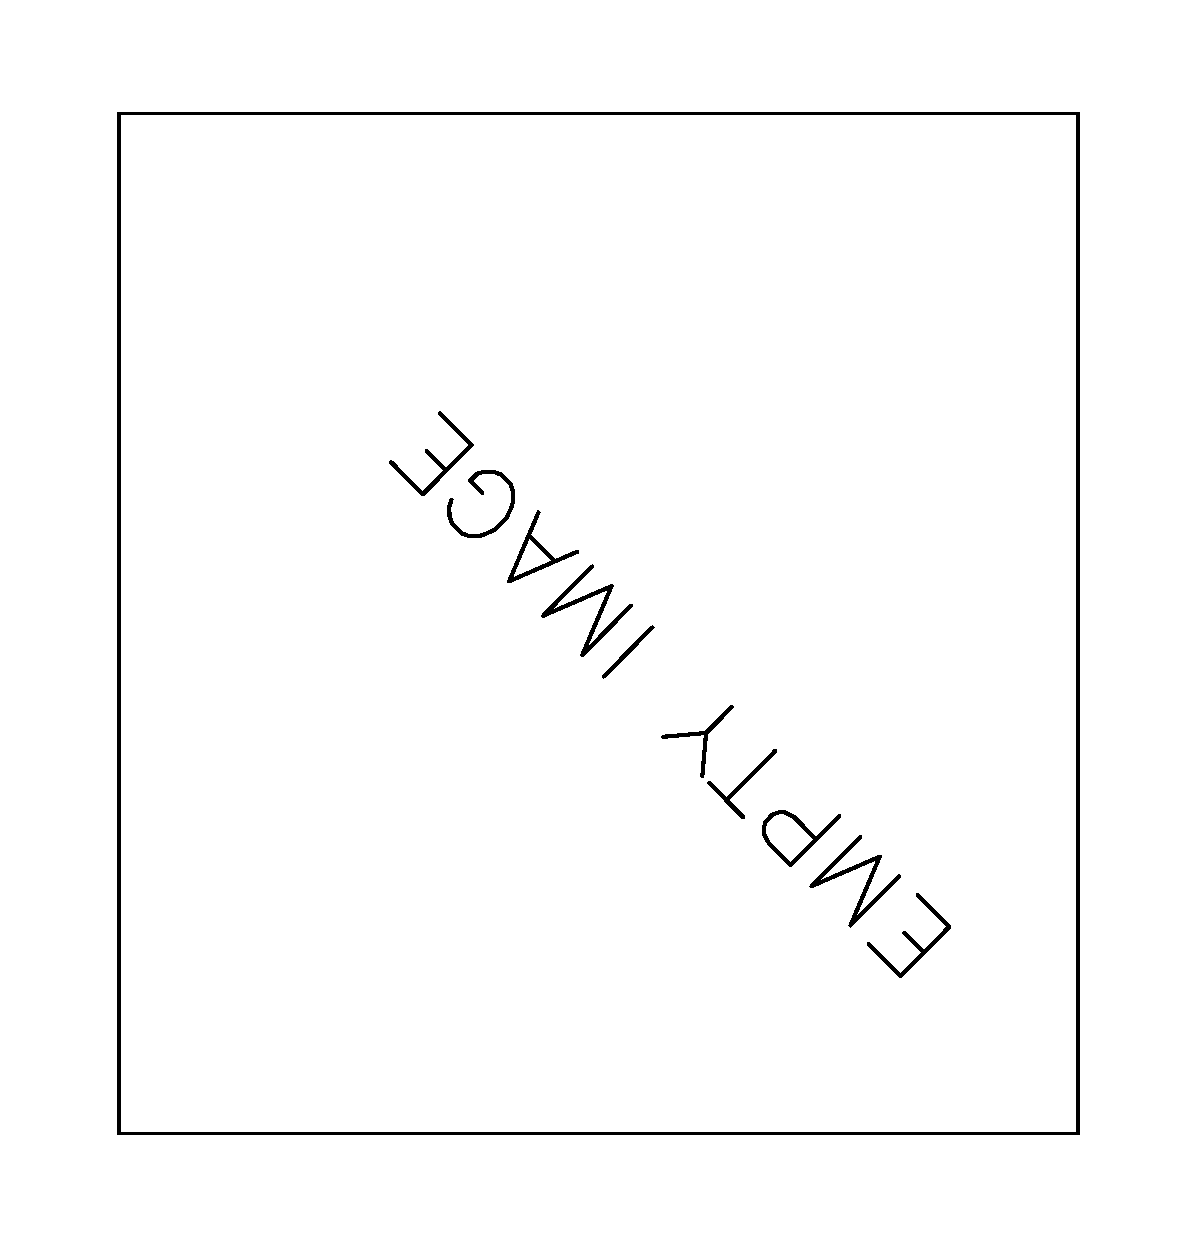
\includegraphics[width=.27\linewidth,angle=-90]{/home/report/FIGS/5GG/1H/emptyimg}}
\subfloat[]{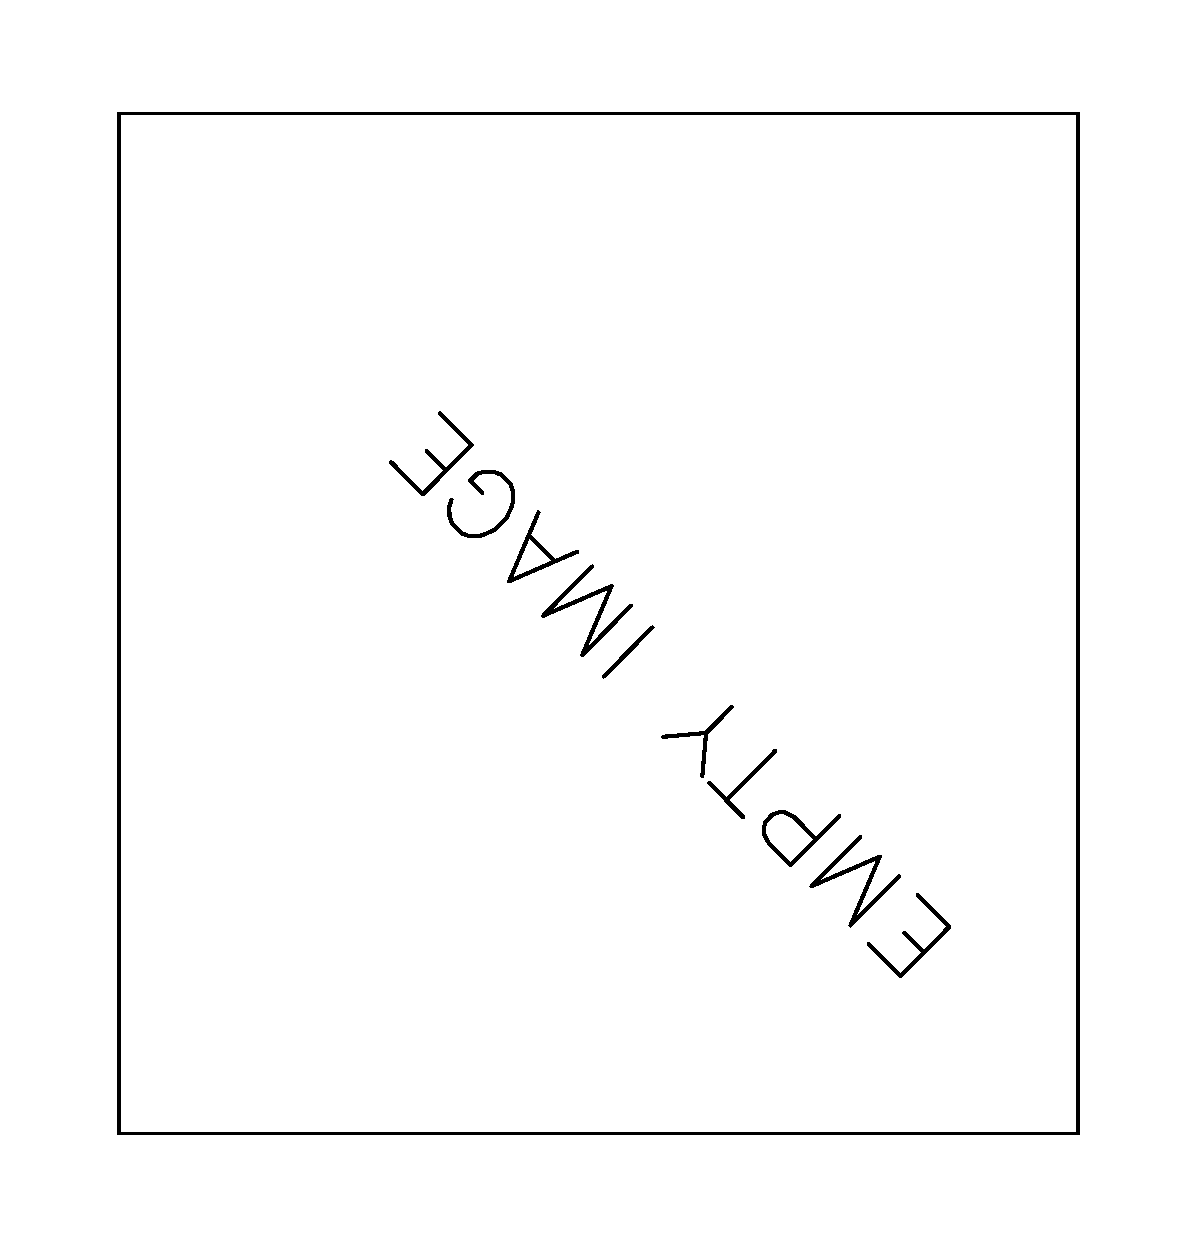
\includegraphics[width=.27\linewidth,angle=-90]{/home/report/FIGS/5GG/1H/emptyimg}}
\caption{TEST-TEST-TEST: (a) STANDARD CONFIGURATION, (b) WITH AR, (c) PERSISTENCE.}
\label{fig:ws}
\end{figure}
%%%%%%%%%%%%%%%%%%%%%%%%%%%%%%%%%
\begin{figure}
\centering
\subfloat[]{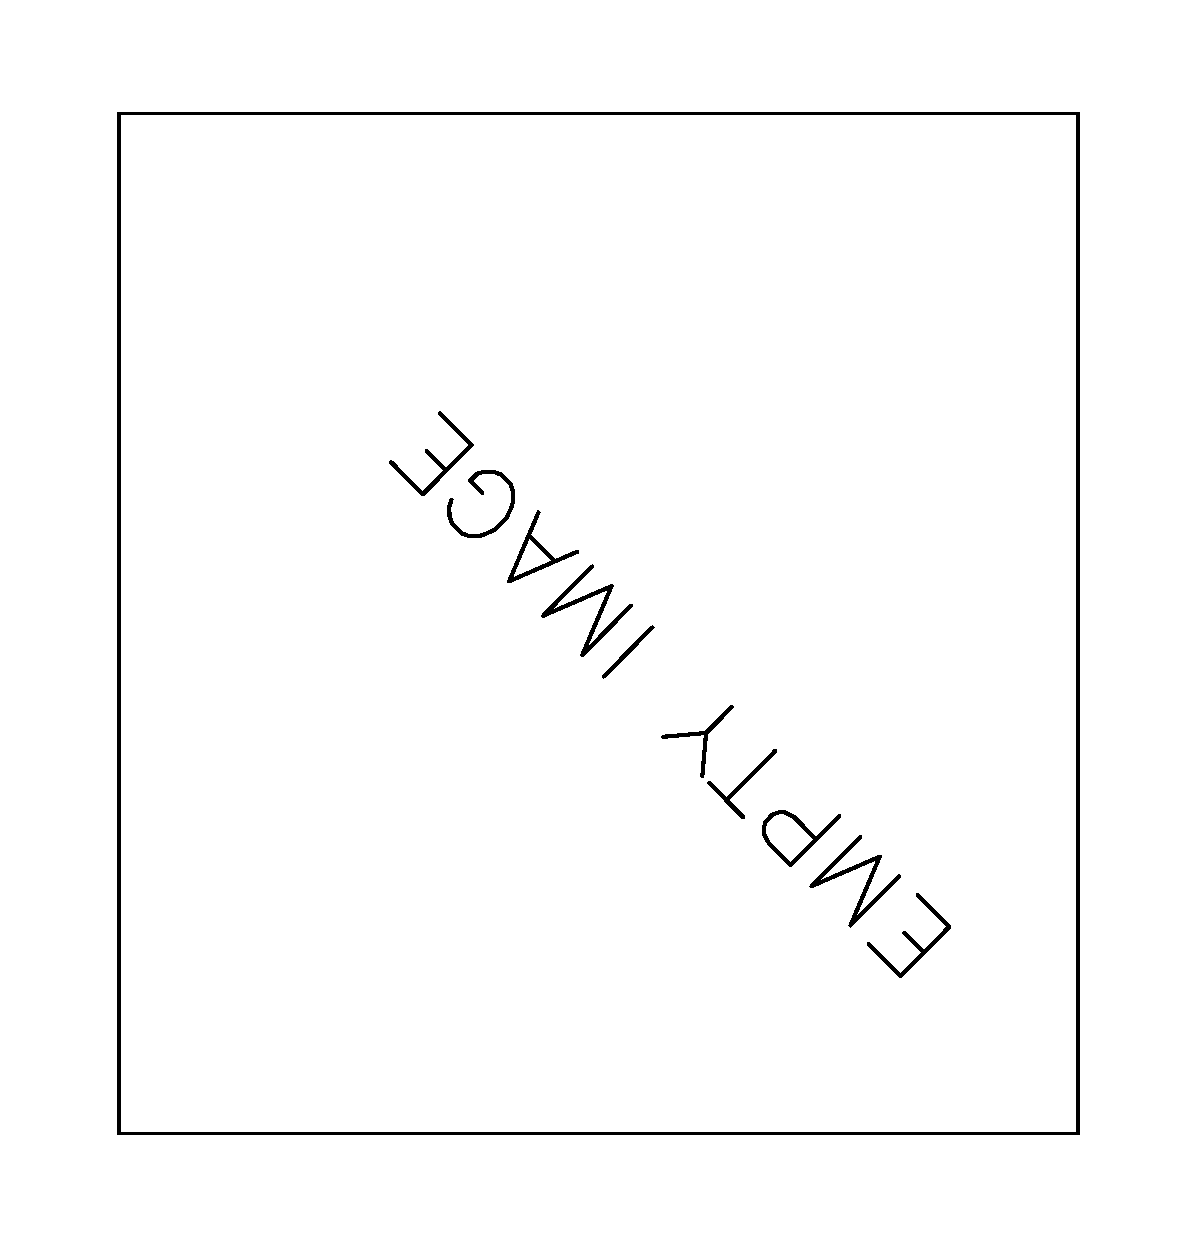
\includegraphics[width=.27\linewidth,angle=-90]{/home/report/FIGS/5GG/1H/emptyimg}}
\subfloat[]{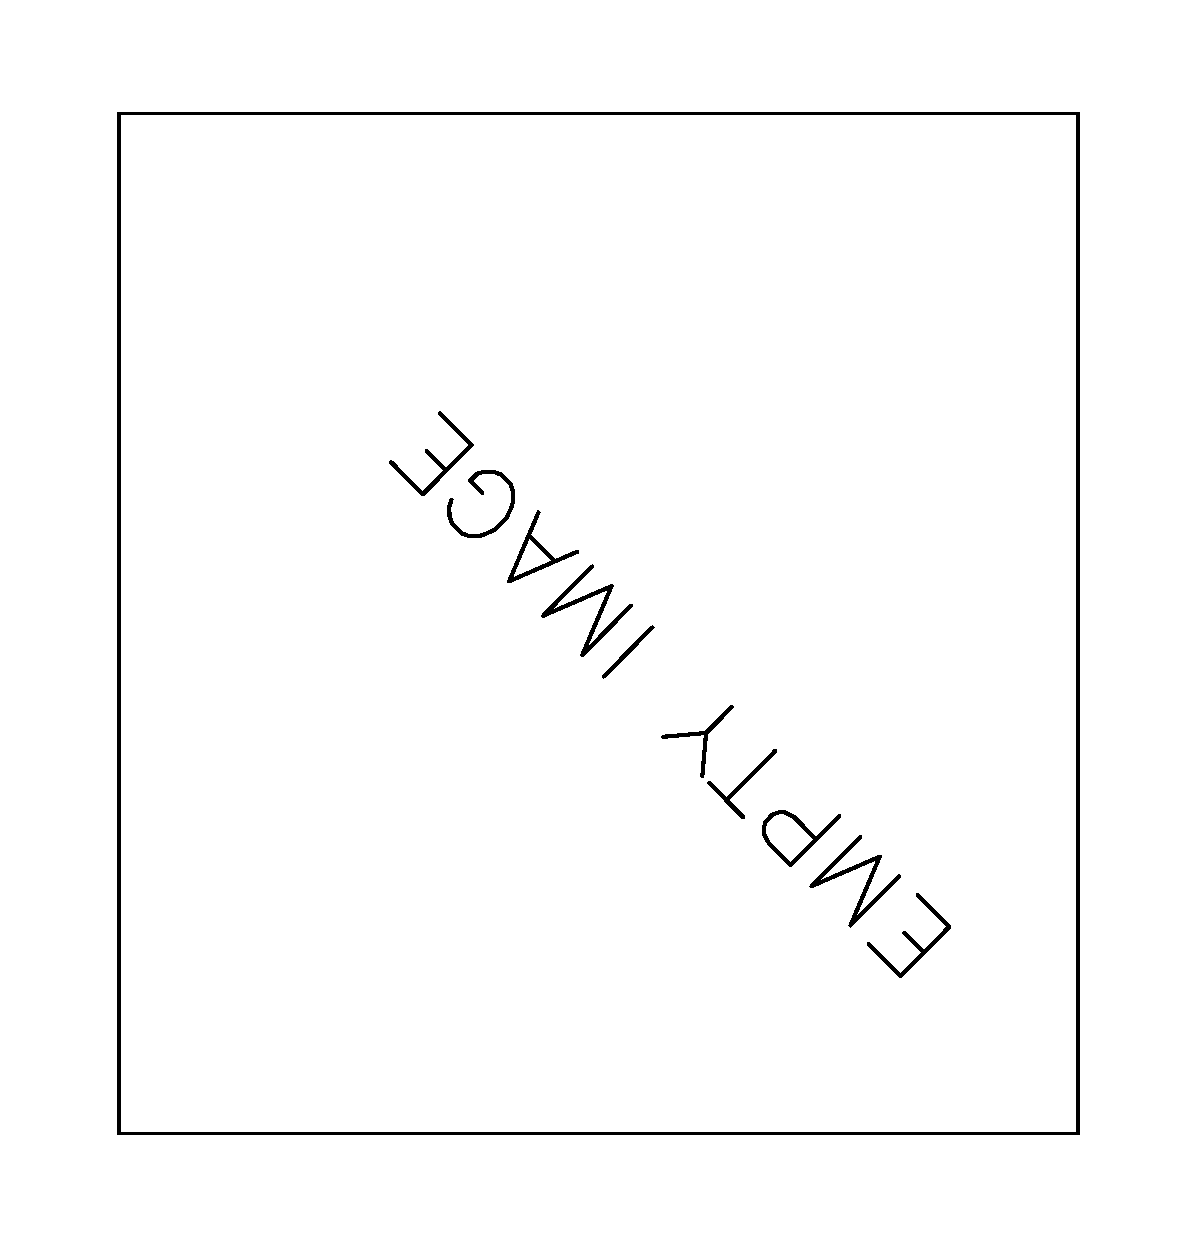
\includegraphics[width=.27\linewidth,angle=-90]{/home/report/FIGS/5GG/1H/emptyimg}}
\subfloat[]{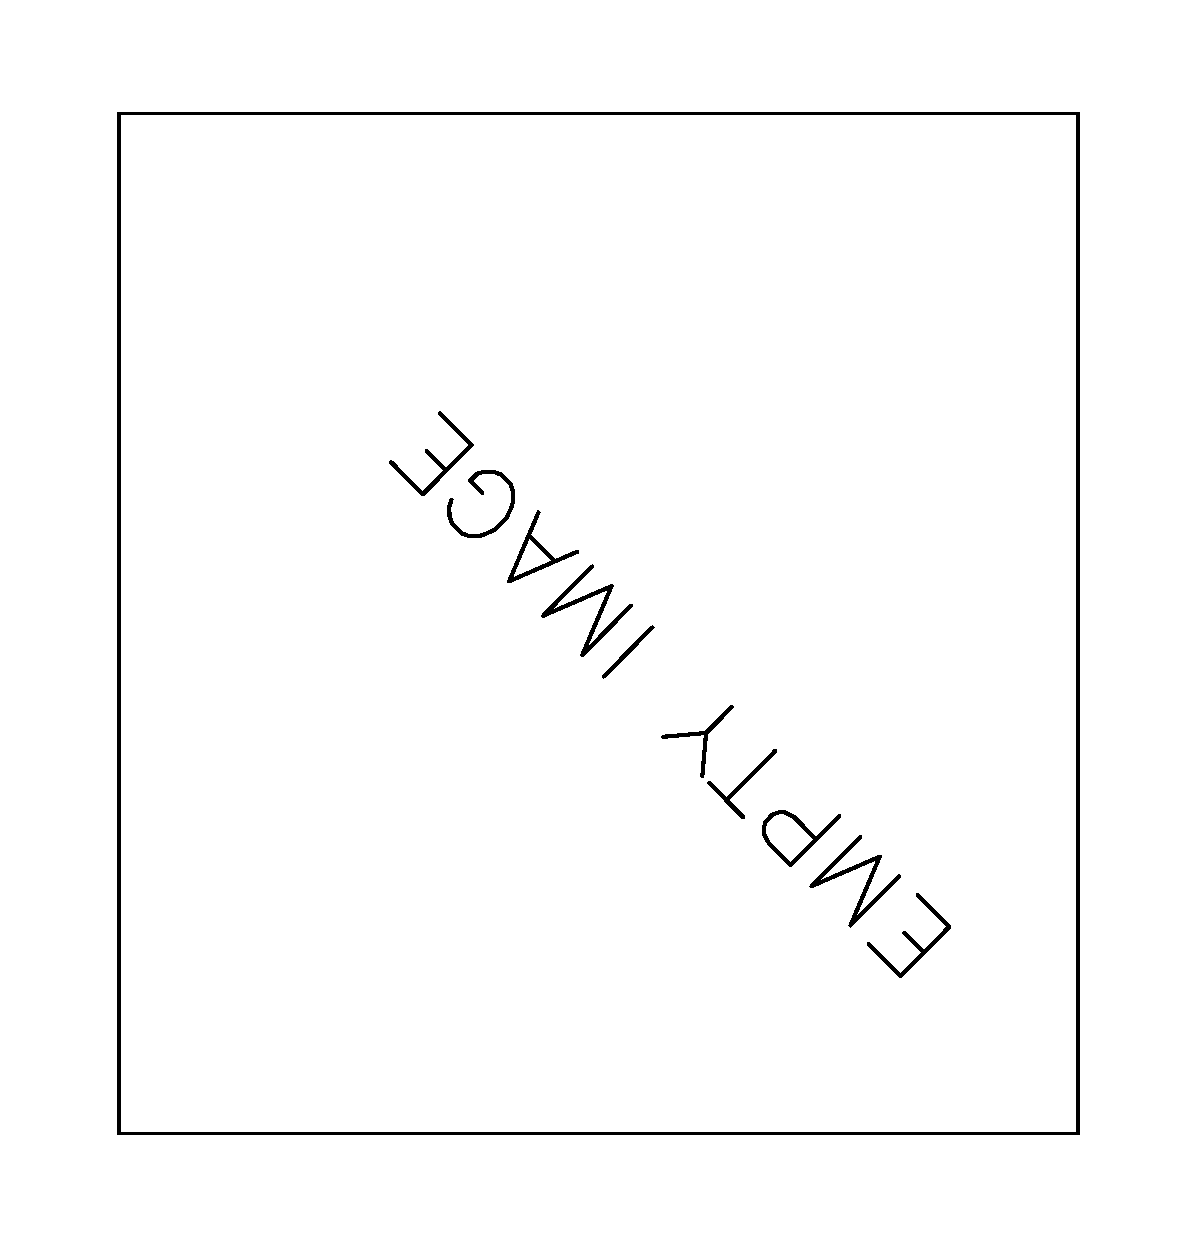
\includegraphics[width=.27\linewidth,angle=-90]{/home/report/FIGS/5GG/1H/emptyimg}}
\caption{TEST-TEST-TEST: (a) STANDARD CONFIGURATION, (b) WITH AR, (c) PERSISTENCE.}
\label{fig:ws}
\end{figure}
%%%%%%%%%%%%%%%%%%%%%%%%%%%%%%%%%
\begin{figure}
\centering
\subfloat[]{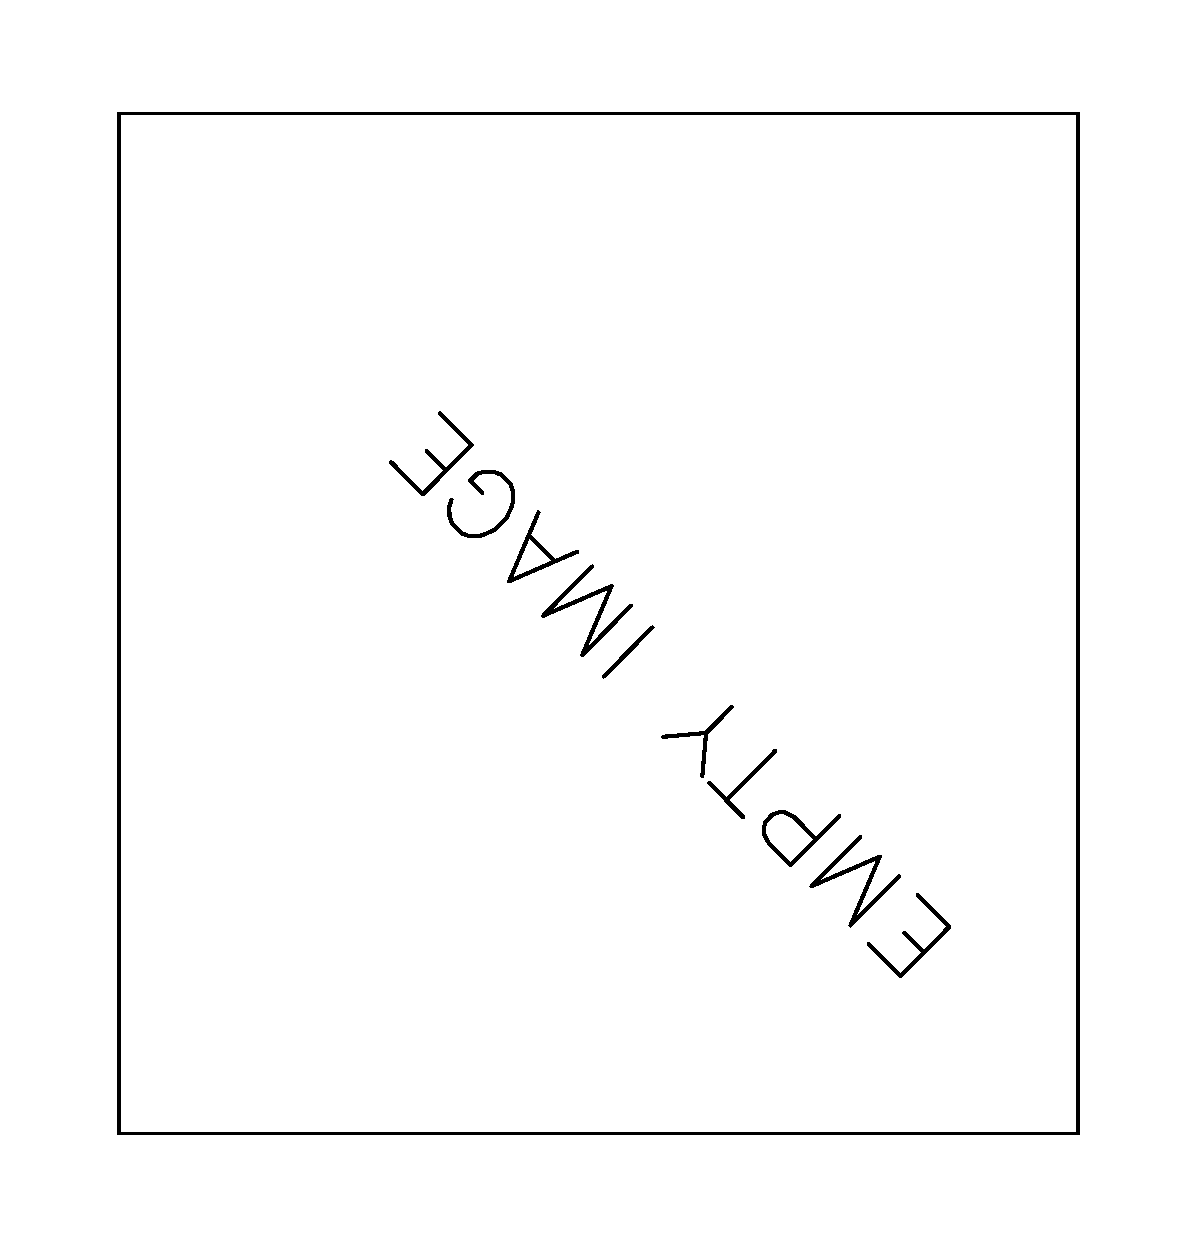
\includegraphics[width=.27\linewidth,angle=-90]{/home/report/FIGS/5GG/1H/emptyimg}}
\subfloat[]{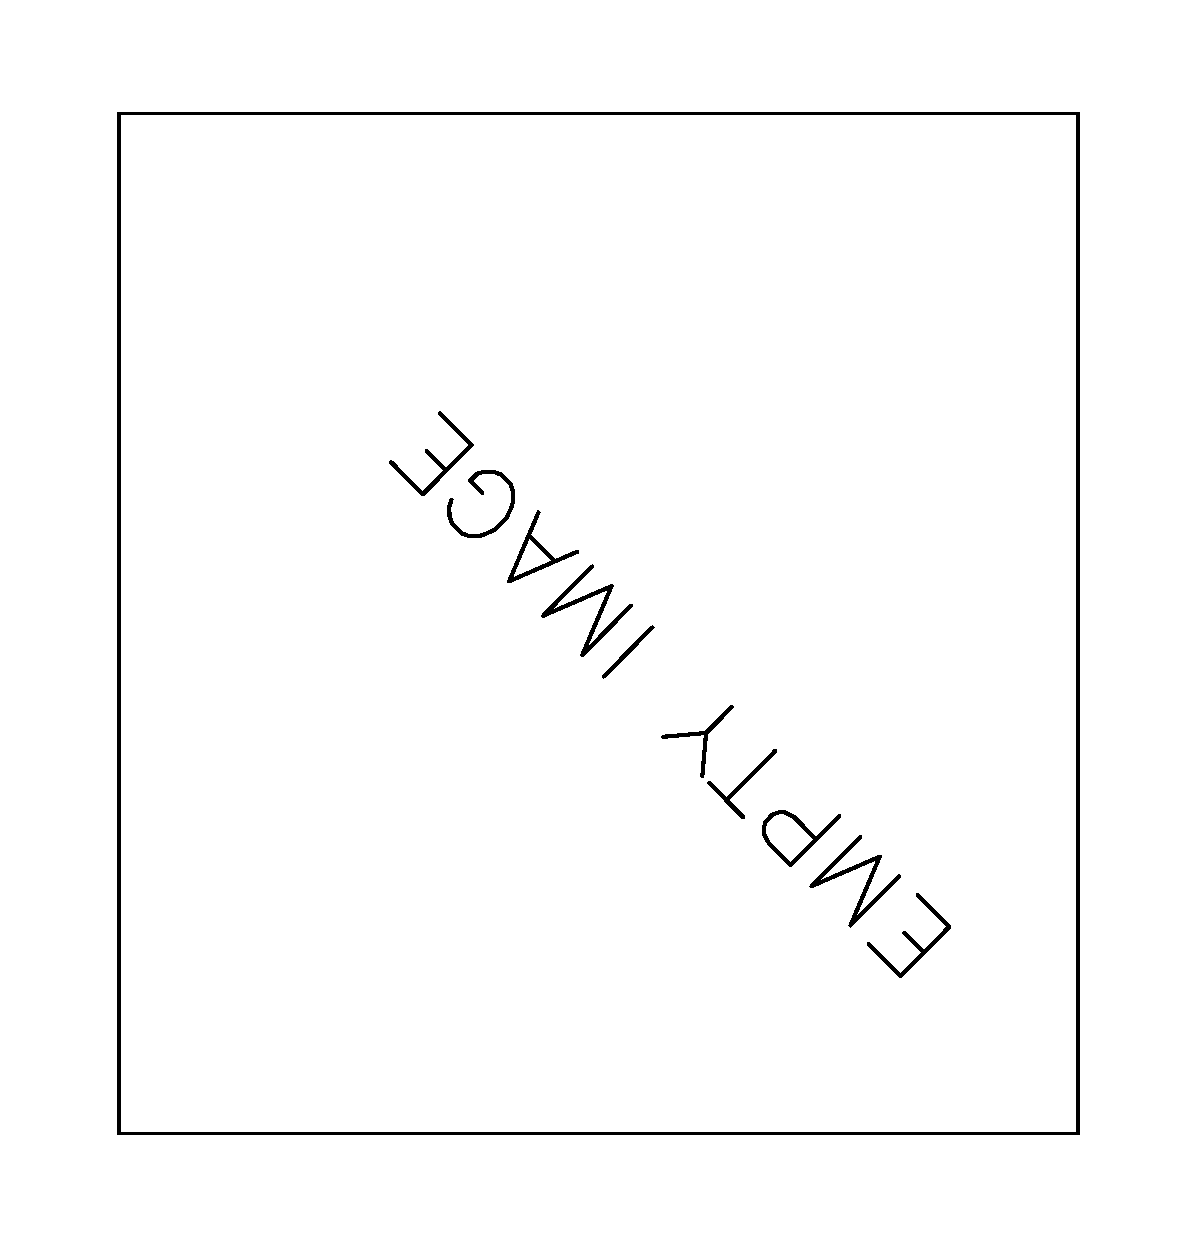
\includegraphics[width=.27\linewidth,angle=-90]{/home/report/FIGS/5GG/1H/emptyimg}}
\subfloat[]{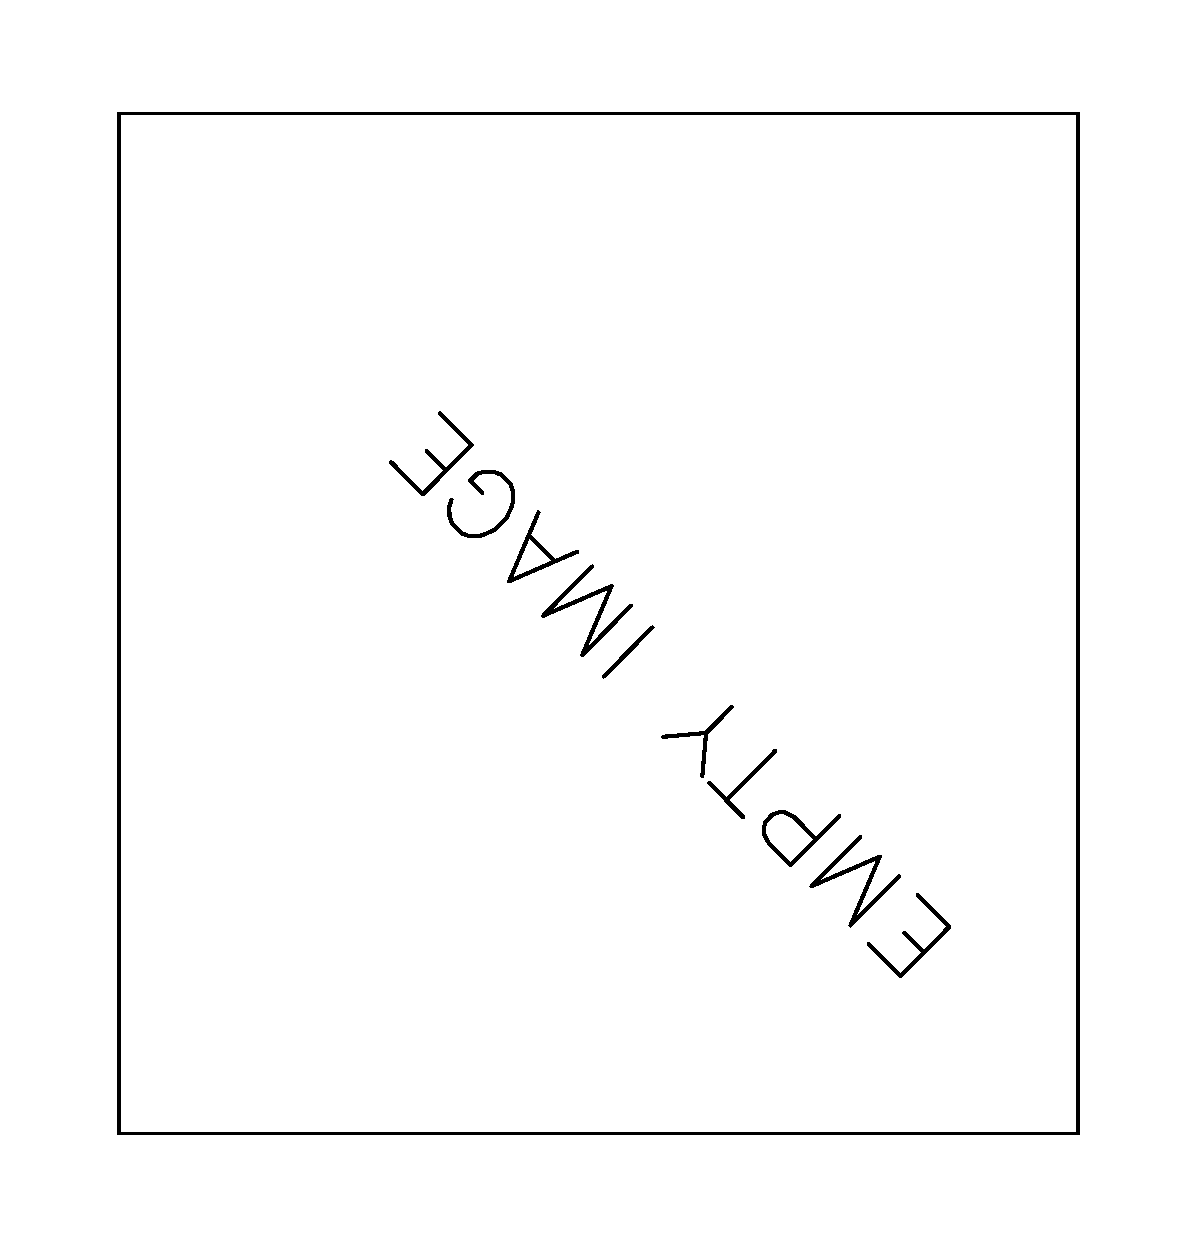
\includegraphics[width=.27\linewidth,angle=-90]{/home/report/FIGS/5GG/1H/emptyimg}}
\caption{TEST-TEST-TEST: (a) STANDARD CONFIGURATION, (b) WITH AR, (c) PERSISTENCE.}
\label{fig:ws}
\end{figure}
%%%%%%%%%%%%%%%%%%%%%%%%%%%%%%%%%
\begin{figure}
\centering
\subfloat[]{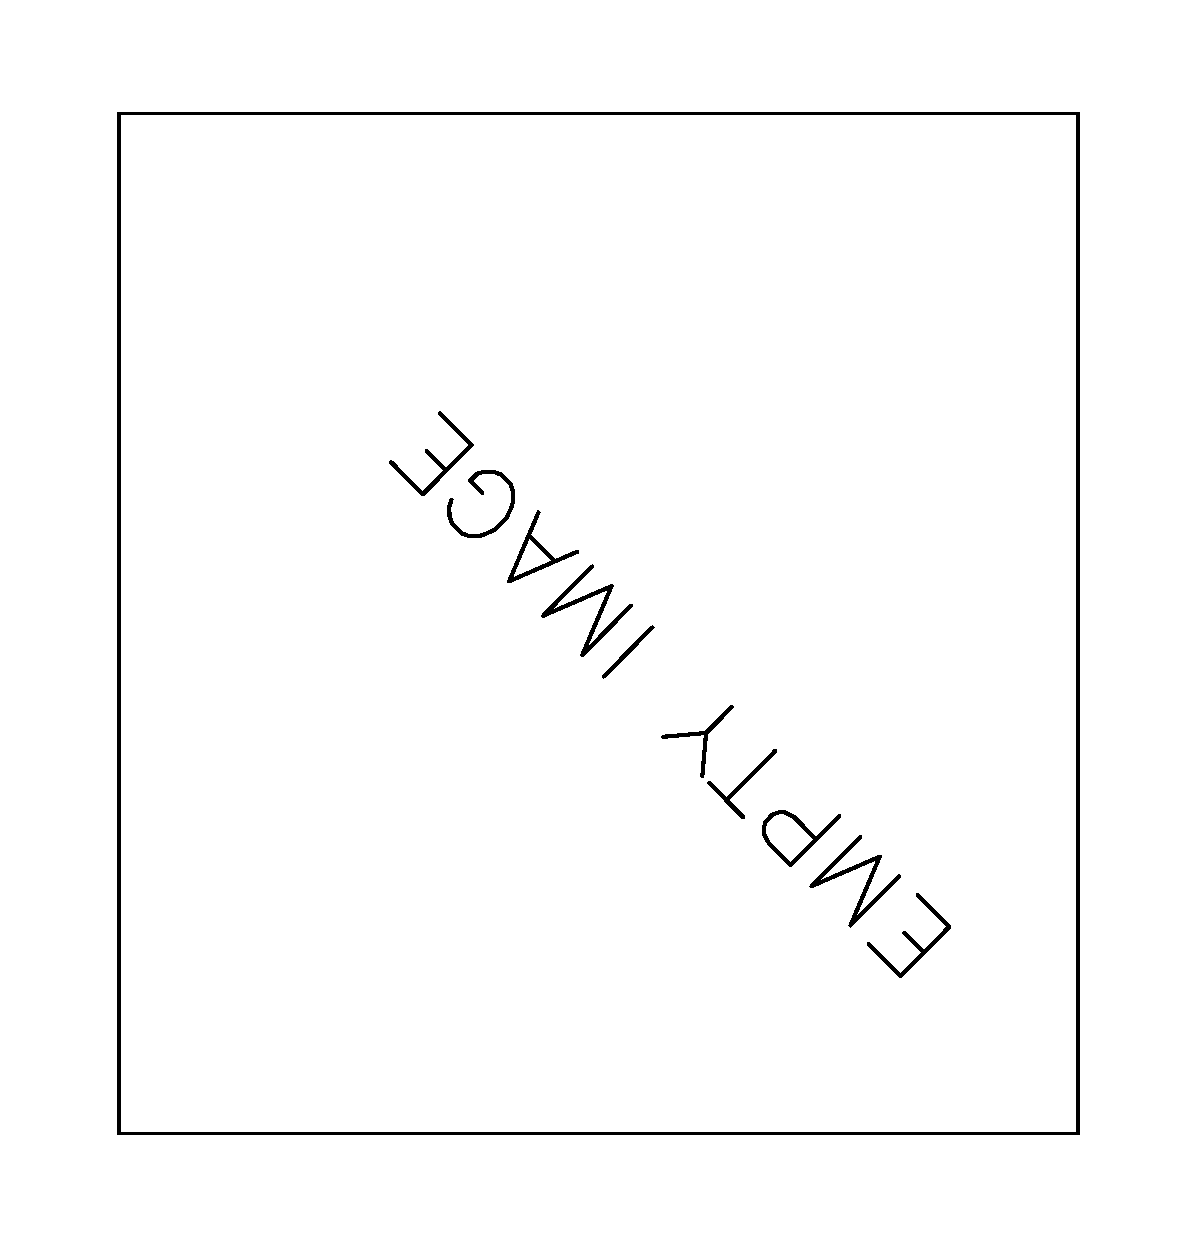
\includegraphics[width=.27\linewidth,angle=-90]{/home/report/FIGS/5GG/1H/emptyimg}}
\subfloat[]{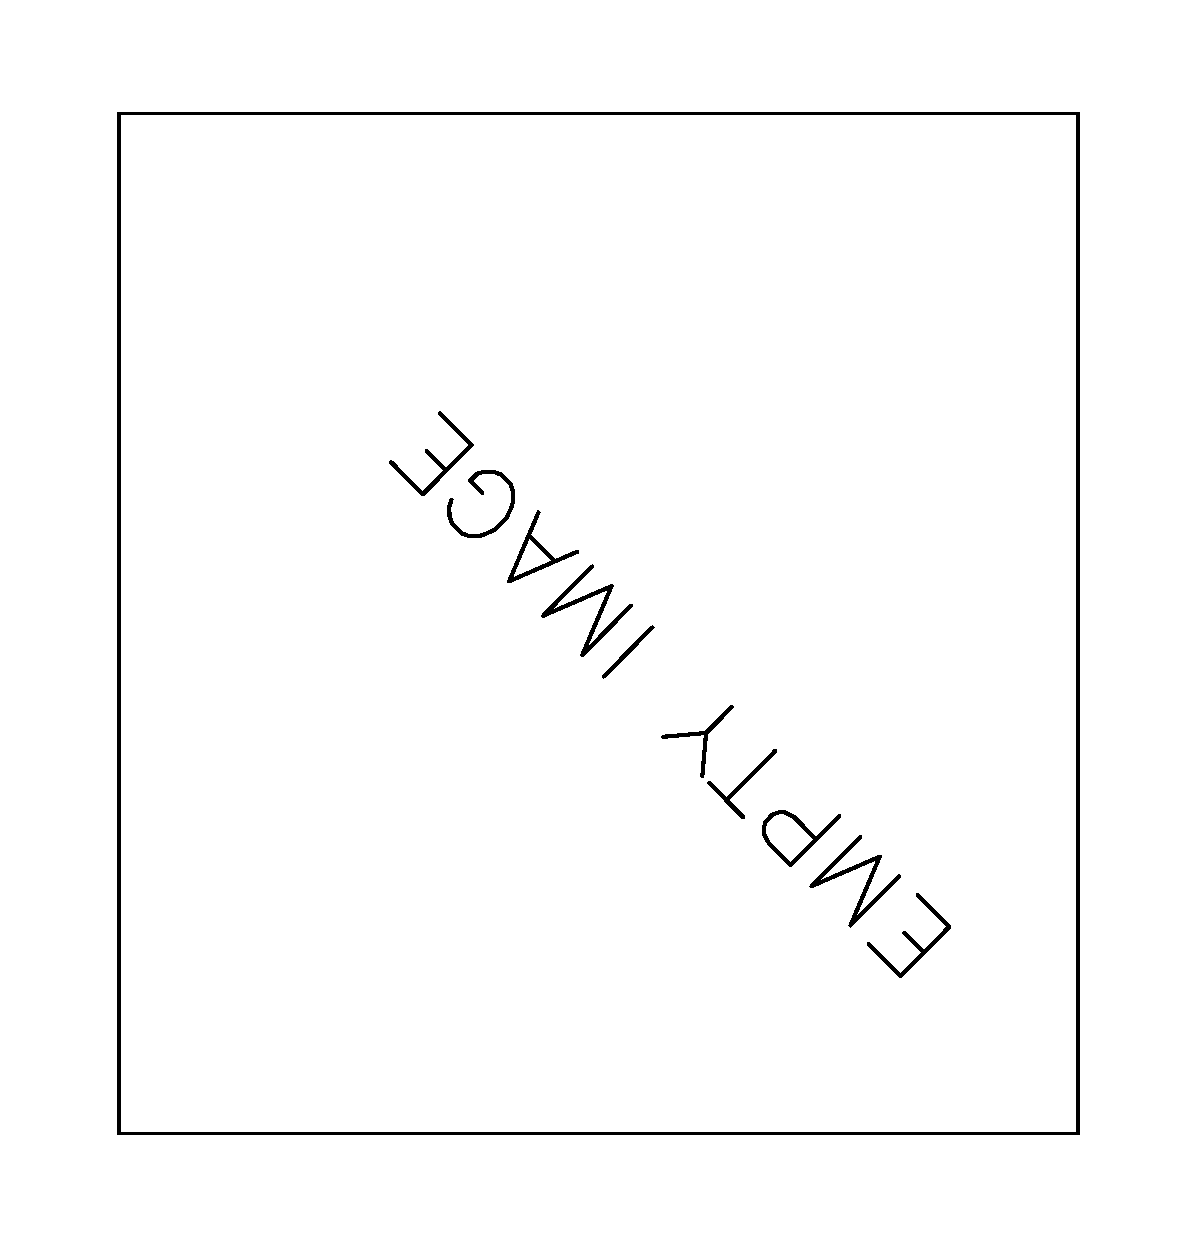
\includegraphics[width=.27\linewidth,angle=-90]{/home/report/FIGS/5GG/1H/emptyimg}}
\subfloat[]{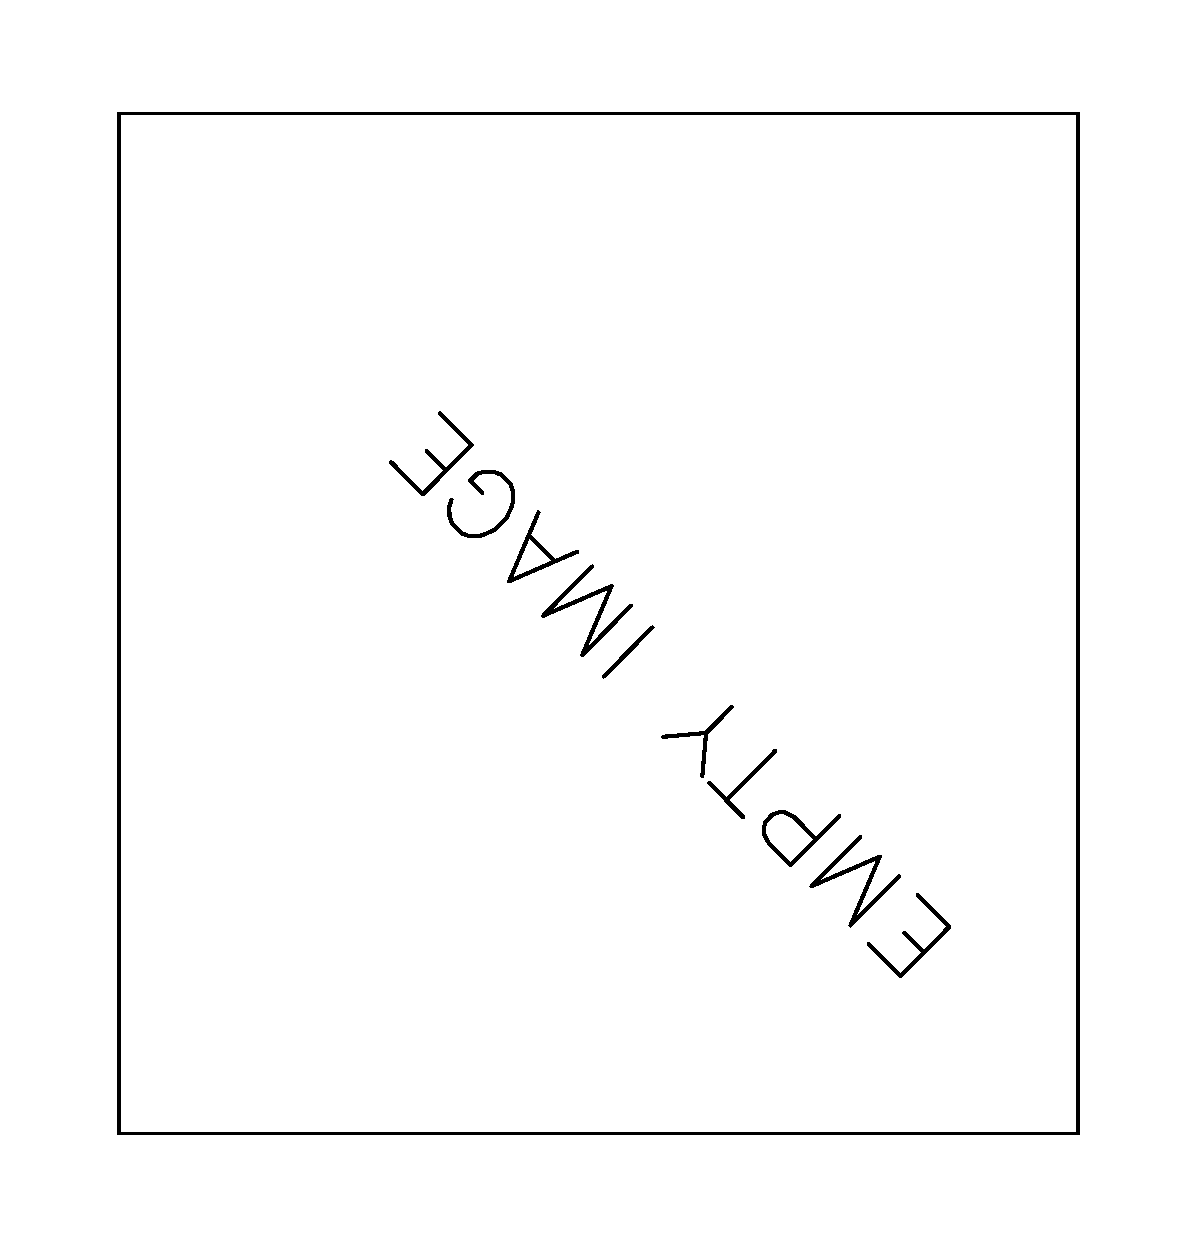
\includegraphics[width=.27\linewidth,angle=-90]{/home/report/FIGS/5GG/1H/emptyimg}}
\caption{TEST-TEST-TEST: (a) STANDARD CONFIGURATION, (b) WITH AR, (c) PERSISTENCE.}
\label{fig:ws}
\end{figure}

%%%%%%%%%%%%%%%%%%%%%%%%%%%%%%%%%
\newpage
%%%%%%%%%%%%%%%%%%%%%%%%%%%%%%%%%

%%%%%%%%%%%%%%%%%%%%
\clearpage
%%%%%%%%%%%%%%%%%%%%
%%%%%%%%%%%%%%%%%%%%%%%%%%%%%%%%%%
%\newpage
\begin{table}[]
\begin{center}
\begin{tabular}{|l|l|l|l|l|}
\hline
\multicolumn{1}{c|}{\cellcolor[HTML]{C0C0C0}\textbf{VARIABLE}} & \multicolumn{1}{c|}{\cellcolor[HTML]{C0C0C0}\textbf{BIAS}} & \multicolumn{1}{c|}{\cellcolor[HTML]{C0C0C0}\textbf{RMSE}} & \multicolumn{1}{c|}{\cellcolor[HTML]{C0C0C0}\textbf{SD}} & \multicolumn{1}{c|}{\cellcolor[HTML]{C0C0C0}\textbf{RMSE-PERS}}\\\hline
\cellcolor[HTML]{C0C0C0}WS  &     0.104                                &     2.487                                &     2.485  &     2.487 \\
\cellcolor[HTML]{C0C0C0}WD  &    -0.973                                &    35.224                                &    35.211  &    35.224 \\
\cellcolor[HTML]{C0C0C0}RH  &     0.735                                &     6.638                                &     6.597  &     6.638 \\
\cellcolor[HTML]{C0C0C0}PWV &    -0.195                               &     1.005                               &     0.986 &     1.005 \\
\cellcolor[HTML]{C0C0C0}SEE &    -0.035                               &     0.331                               &     0.330 &     0.333 \\
\cellcolor[HTML]{C0C0C0}TAU &    -0.073                               &     2.221                               &     2.220 &     2.189 \\
\cellcolor[HTML]{C0C0C0}GLF &    -0.147                               &     0.264                               &     0.219 &     0.233 \\
\hline
\end{tabular}
\caption{Statistics for variables in standard configuration (i.e. BEF)}
\end{center}
\end{table}
%%%%%%%%%%%%%%%%%%%%%%%%%%%%%%%%%%
%\newpage
\begin{table}[]
\begin{center}
\begin{tabular}{|l|l|l|l|l|}
\hline
\multicolumn{1}{c|}{\cellcolor[HTML]{C0C0C0}\textbf{VARIABLE}} & \multicolumn{1}{c|}{\cellcolor[HTML]{C0C0C0}\textbf{BIAS}} & \multicolumn{1}{c|}{\cellcolor[HTML]{C0C0C0}\textbf{RMSE}} & \multicolumn{1}{c|}{\cellcolor[HTML]{C0C0C0}\textbf{SD}} & \multicolumn{1}{c|}{\cellcolor[HTML]{C0C0C0}\textbf{RMSE-PERS}}\\\hline
\cellcolor[HTML]{C0C0C0}WS  &    -0.010                                &     0.659                                &     0.659  &     0.918 \\
\cellcolor[HTML]{C0C0C0}WD  &     0.298                                &     6.650                                &     6.644  &    12.471 \\
\cellcolor[HTML]{C0C0C0}RH  &    -0.012                                &     1.368                                &     1.368  &     2.178 \\
\cellcolor[HTML]{C0C0C0}PWV &    -0.007                               &     0.125                               &     0.125 &     0.252 \\
\cellcolor[HTML]{C0C0C0}SEE &    -0.000                               &     0.105                               &     0.105 &     0.155 \\
\cellcolor[HTML]{C0C0C0}TAU &    -0.022                               &     0.618                               &     0.618 &     1.058 \\
\cellcolor[HTML]{C0C0C0}GLF &    -0.007                               &     0.067                               &     0.067 &     0.093 \\
\hline
\end{tabular}
\caption{Statistics for variables processed with AR (i.e. AFT)}
\end{center}
\end{table}

%%%%%%%%%%%%%%%%%%%%%%%%%%%%%%%%%
\newpage
%%%%%%%%%%%%%%%%%%%%%%%%%%%%%%%%%

%%%%%%%%%%%%%%%%%%%%
\clearpage
%%%%%%%%%%%%%%%%%%%%
%%%%%%%%%%%%%%%%%%%%%%%%%%%%%%%%%
\begin{table}[]
\begin{center}
\begin{tabular}{llccc}
\hline
{Wind speed}                                       &                                                    & \multicolumn{3}{c}{Observations}                 \\
{$m s^{-1}$}                                       &                             & ws $<$ 4.2   & 4.2 $<$ ws $<$ 7.5 & ws $>$ 7.5 \\
\hline
\multicolumn{1}{c}{\multirow{3}{*}{Model data}}  & ws $<$ 4.2             & 4541                & 2127                       & 249              \\
                                                 & 4.2  $<$ ws $<$ 7.5 & 3034                & 3970                       & 1347              \\
                                                 & ws $>$ 7.5             & 430                & 1908                       & 6408              \\
\hline
\end{tabular}
\end{center}
\caption{Contingency table for variable Wind speed ($m s^{-1}$) in standard configuration (i.e. BEF)}
\label{tab:contingencywsBEF}
\end{table}
%%%%%%%%%%%%%%%%%%%%%%%%%%%%%%%%%
\begin{table}[]
\begin{center}
\begin{tabular}{llccc}
\hline
{Wind speed}                                       &                                                    & \multicolumn{3}{c}{Observations}                 \\
{$m s^{-1}$}                                       &                             & ws $<$ 4.2   & 4.2 $<$ ws $<$ 7.5 & ws $>$ 7.5 \\
\hline
\multicolumn{1}{c}{\multirow{3}{*}{Model data}}  & ws $<$ 4.2             & 7377                & 623                       & 1              \\
                                                 & 4.2  $<$ ws $<$ 7.5 & 628                & 6950                       & 386              \\
                                                 & ws $>$ 7.5             & 0                & 432                       & 7617              \\
\hline
\end{tabular}
\end{center}
\caption{Contingency table for variable Wind speed ($m s^{-1}$) processed with AR (i.e. AFT)}
\label{tab:contingencywsAFT}
\end{table}
%%%%%%%%%%%%%%%%%%%%%%%%%%%%%%%%%
\begin{table}[]
\begin{center}
\begin{tabular}{llccc}
\hline
{Relative humidity}                                       &                                                    & \multicolumn{3}{c}{Observations}                 \\
{percent}                                       &                             & rh $<$ 7.1   & 7.1 $<$ rh $<$ 15.3 & rh $>$ 15.3 \\
\hline
\multicolumn{1}{c}{\multirow{3}{*}{Model data}}  & rh $<$ 7.1             & 4755                & 1095                       & 27              \\
                                                 & 7.1  $<$ rh $<$ 15.3 & 2696                & 5193                       & 1357              \\
                                                 & rh $>$ 15.3             & 379                & 1539                       & 6443              \\
\hline
\end{tabular}
\end{center}
\caption{Contingency table for variable Relative humidity (percent) in standard configuration (i.e. BEF)}
\label{tab:contingencyrhBEF}
\end{table}
%%%%%%%%%%%%%%%%%%%%%%%%%%%%%%%%%
\begin{table}[]
\begin{center}
\begin{tabular}{llccc}
\hline
{Relative humidity}                                       &                                                    & \multicolumn{3}{c}{Observations}                 \\
{percent}                                       &                             & rh $<$ 7.1   & 7.1 $<$ rh $<$ 15.3 & rh $>$ 15.3 \\
\hline
\multicolumn{1}{c}{\multirow{3}{*}{Model data}}  & rh $<$ 7.1             & 7408                & 328                       & 1              \\
                                                 & 7.1  $<$ rh $<$ 15.3 & 422                & 7294                       & 248              \\
                                                 & rh $>$ 15.3             & 0                & 205                       & 7578              \\
\hline
\end{tabular}
\end{center}
\caption{Contingency table for variable Relative humidity (percent) processed with AR (i.e. AFT)}
\label{tab:contingencyrhAFT}
\end{table}
%%%%%%%%%%%%%%%%%%%%%%%%%%%%%%%%%
\begin{table}[]
\begin{center}
\begin{tabular}{llccc}
\hline
{Precipitable water vapor}                                       &                                                    & \multicolumn{3}{c}{Observations}                 \\
{mm}                                       &                             & pwv $<$ 1.9   & 1.9 $<$ pwv $<$ 3.5 & pwv $>$ 3.5 \\
\hline
\multicolumn{1}{c}{\multirow{3}{*}{Model data}}  & pwv $<$ 1.9             & 3402                & 854                       & 2              \\
                                                 & 1.9  $<$ pwv $<$ 3.5 & 443                & 2596                       & 576              \\
                                                 & pwv $>$ 3.5             & 5                & 400                       & 3271              \\
\hline
\end{tabular}
\end{center}
\caption{Contingency table for variable Precipitable water vapor (mm) in standard configuration (i.e. BEF)}
\label{tab:contingencypwvBEF}
\end{table}
%%%%%%%%%%%%%%%%%%%%%%%%%%%%%%%%%
\begin{table}[]
\begin{center}
\begin{tabular}{llccc}
\hline
{Precipitable water vapor}                                       &                                                    & \multicolumn{3}{c}{Observations}                 \\
{mm}                                       &                             & pwv $<$ 1.9   & 1.9 $<$ pwv $<$ 3.5 & pwv $>$ 3.5 \\
\hline
\multicolumn{1}{c}{\multirow{3}{*}{Model data}}  & pwv $<$ 1.9             & 3785                & 69                       & 0              \\
                                                 & 1.9  $<$ pwv $<$ 3.5 & 65                & 3733                       & 39              \\
                                                 & pwv $>$ 3.5             & 0                & 48                       & 3810              \\
\hline
\end{tabular}
\end{center}
\caption{Contingency table for variable Precipitable water vapor (mm) processed with AR (i.e. AFT)}
\label{tab:contingencypwvAFT}
\end{table}
%%%%%%%%%%%%%%%%%%%%
\clearpage
%%%%%%%%%%%%%%%%%%%%
%%%%%%%%%%%%%%%%%%%%%%%%%%%%%%%%%
\begin{table}[]
\begin{center}
\begin{tabular}{llccc}
\hline
{Total seeing}                                       &                                                    & \multicolumn{3}{c}{Observations}                 \\
{arcsec}                                       &                             & see $<$ 0.6   & 0.6 $<$ see $<$ 0.8 & see $>$ 0.8 \\
\hline
\multicolumn{1}{c}{\multirow{3}{*}{Model data}}  & see $<$ 0.6             & 2937                & 1831                       & 506              \\
                                                 & 0.6  $<$ see $<$ 0.8 & 2926                & 3110                       & 2000              \\
                                                 & see $>$ 0.8             & 583                & 1505                       & 3940              \\
\hline
\end{tabular}
\end{center}
\caption{Contingency table for variable Total seeing (arcsec) in standard configuration (i.e. BEF) and accuracy 0.0}
\label{tab:contingencyseeBEF}
\end{table}
%%%%%%%%%%%%%%%%%%%%%%%%%%%%%%%%%
\begin{table}[]
\begin{center}
\begin{tabular}{llccc}
\hline
{Total seeing}                                       &                                                    & \multicolumn{3}{c}{Observations}                 \\
{arcsec}                                       &                             & see $<$ 0.6   & 0.6 $<$ see $<$ 0.8 & see $>$ 0.8 \\
\hline
\multicolumn{1}{c}{\multirow{3}{*}{Model data}}  & see $<$ 0.6             & 2937                & 1831                       & 506              \\
                                                 & 0.6  $<$ see $<$ 0.8 & 2926                & 3110                       & 2000              \\
                                                 & see $>$ 0.8             & 583                & 1505                       & 3940              \\
\hline
\end{tabular}
\end{center}
\caption{Contingency table for variable Total seeing (arcsec) in standard configuration (i.e. BEF) and accuracy 0.10}
\label{tab:contingencyseeBEF}
\end{table}
%%%%%%%%%%%%%%%%%%%%%%%%%%%%%%%%%
\begin{table}[]
\begin{center}
\begin{tabular}{llccc}
\hline
{Total seeing}                                       &                                                    & \multicolumn{3}{c}{Observations}                 \\
{arcsec}                                       &                             & see $<$ 0.6   & 0.6 $<$ see $<$ 0.8 & see $>$ 0.8 \\
\hline
\multicolumn{1}{c}{\multirow{3}{*}{Model data}}  & see $<$ 0.6             & 2937                & 1831                       & 506              \\
                                                 & 0.6  $<$ see $<$ 0.8 & 2926                & 3110                       & 2000              \\
                                                 & see $>$ 0.8             & 583                & 1505                       & 3940              \\
\hline
\end{tabular}
\end{center}
\caption{Contingency table for variable Total seeing (arcsec) in standard configuration (i.e. BEF) and accuracy 0.24}
\label{tab:contingencyseeBEF}
\end{table}
%%%%%%%%%%%%%%%%%%%%%%%%%%%%%%%%%
\begin{table}[]
\begin{center}
\begin{tabular}{llccc}
\hline
{Total seeing}                                       &                                                    & \multicolumn{3}{c}{Observations}                 \\
{arcsec}                                       &                             & see $<$ 0.6   & 0.6 $<$ see $<$ 0.8 & see $>$ 0.8 \\
\hline
\multicolumn{1}{c}{\multirow{3}{*}{Model data}}  & see $<$ 0.6             & 5670                & 816                       & 27              \\
                                                 & 0.6  $<$ see $<$ 0.8 & 765                & 4910                       & 535              \\
                                                 & see $>$ 0.8             & 11                & 720                       & 5884              \\
\hline
\end{tabular}
\end{center}
\caption{Contingency table for variable Total seeing (arcsec) processed with AR (i.e. AFT) and accuracy 0.0}
\label{tab:contingencyseeAFT}
\end{table}
%%%%%%%%%%%%%%%%%%%%%%%%%%%%%%%%%
\begin{table}[]
\begin{center}
\begin{tabular}{llccc}
\hline
{Total seeing}                                       &                                                    & \multicolumn{3}{c}{Observations}                 \\
{arcsec}                                       &                             & see $<$ 0.6   & 0.6 $<$ see $<$ 0.8 & see $>$ 0.8 \\
\hline
\multicolumn{1}{c}{\multirow{3}{*}{Model data}}  & see $<$ 0.6             & 5670                & 816                       & 27              \\
                                                 & 0.6  $<$ see $<$ 0.8 & 765                & 4910                       & 535              \\
                                                 & see $>$ 0.8             & 11                & 720                       & 5884              \\
\hline
\end{tabular}
\end{center}
\caption{Contingency table for variable Total seeing (arcsec) processed with AR (i.e. AFT) and accuracy 0.10}
\label{tab:contingencyseeAFT}
\end{table}
%%%%%%%%%%%%%%%%%%%%%%%%%%%%%%%%%
\begin{table}[]
\begin{center}
\begin{tabular}{llccc}
\hline
{Total seeing}                                       &                                                    & \multicolumn{3}{c}{Observations}                 \\
{arcsec}                                       &                             & see $<$ 0.6   & 0.6 $<$ see $<$ 0.8 & see $>$ 0.8 \\
\hline
\multicolumn{1}{c}{\multirow{3}{*}{Model data}}  & see $<$ 0.6             & 5670                & 816                       & 27              \\
                                                 & 0.6  $<$ see $<$ 0.8 & 765                & 4910                       & 535              \\
                                                 & see $>$ 0.8             & 11                & 720                       & 5884              \\
\hline
\end{tabular}
\end{center}
\caption{Contingency table for variable Total seeing (arcsec) processed with AR (i.e. AFT) and accuracy 0.24}
\label{tab:contingencyseeAFT}
\end{table}
%%%%%%%%%%%%%%%%%%%%%%%%%%%%%%%%%
\begin{table}[]
\begin{center}
\begin{tabular}{llccc}
\hline
{Coeherence time}                                       &                                                    & \multicolumn{3}{c}{Observations}                 \\
{ms}                                       &                             & tau $<$ 3.4   & 3.4 $<$ tau $<$ 5.8 & tau $>$ 5.8 \\
\hline
\multicolumn{1}{c}{\multirow{3}{*}{Model data}}  & tau $<$ 3.4             & 3678                & 872                       & 99              \\
                                                 & 3.4  $<$ tau $<$ 5.8 & 1794                & 3570                       & 2015              \\
                                                 & tau $>$ 5.8             & 281                & 1311                       & 3639              \\
\hline
\end{tabular}
\end{center}
\caption{Contingency table for variable Coeherence time (ms) in standard configuration (i.e. BEF) and accuracy 0.0}
\label{tab:contingencytauBEF}
\end{table}
%%%%%%%%%%%%%%%%%%%%%%%%%%%%%%%%%
\begin{table}[]
\begin{center}
\begin{tabular}{llccc}
\hline
{Coeherence time}                                       &                                                    & \multicolumn{3}{c}{Observations}                 \\
{ms}                                       &                             & tau $<$ 3.4   & 3.4 $<$ tau $<$ 5.8 & tau $>$ 5.8 \\
\hline
\multicolumn{1}{c}{\multirow{3}{*}{Model data}}  & tau $<$ 3.4             & 3678                & 872                       & 99              \\
                                                 & 3.4  $<$ tau $<$ 5.8 & 1794                & 3570                       & 2015              \\
                                                 & tau $>$ 5.8             & 281                & 1311                       & 3639              \\
\hline
\end{tabular}
\end{center}
\caption{Contingency table for variable Coeherence time (ms) in standard configuration (i.e. BEF) and accuracy 1.22}
\label{tab:contingencytauBEF}
\end{table}
%%%%%%%%%%%%%%%%%%%%%%%%%%%%%%%%%
\begin{table}[]
\begin{center}
\begin{tabular}{llccc}
\hline
{Coeherence time}                                       &                                                    & \multicolumn{3}{c}{Observations}                 \\
{ms}                                       &                             & tau $<$ 3.4   & 3.4 $<$ tau $<$ 5.8 & tau $>$ 5.8 \\
\hline
\multicolumn{1}{c}{\multirow{3}{*}{Model data}}  & tau $<$ 3.4             & 5349                & 369                       & 1              \\
                                                 & 3.4  $<$ tau $<$ 5.8 & 401                & 4970                       & 417              \\
                                                 & tau $>$ 5.8             & 3                & 414                       & 5335              \\
\hline
\end{tabular}
\end{center}
\caption{Contingency table for variable Coeherence time (ms) processed with AR (i.e. AFT) and accuracy 0.0}
\label{tab:contingencytauAFT}
\end{table}
%%%%%%%%%%%%%%%%%%%%%%%%%%%%%%%%%
\begin{table}[]
\begin{center}
\begin{tabular}{llccc}
\hline
{Coeherence time}                                       &                                                    & \multicolumn{3}{c}{Observations}                 \\
{ms}                                       &                             & tau $<$ 3.4   & 3.4 $<$ tau $<$ 5.8 & tau $>$ 5.8 \\
\hline
\multicolumn{1}{c}{\multirow{3}{*}{Model data}}  & tau $<$ 3.4             & 5349                & 369                       & 1              \\
                                                 & 3.4  $<$ tau $<$ 5.8 & 401                & 4970                       & 417              \\
                                                 & tau $>$ 5.8             & 3                & 414                       & 5335              \\
\hline
\end{tabular}
\end{center}
\caption{Contingency table for variable Coeherence time (ms) processed with AR (i.e. AFT) and accuracy 1.22}
\label{tab:contingencytauAFT}
\end{table}
%%%%%%%%%%%%%%%%%%%%%%%%%%%%%%%%%
\begin{table}[]
\begin{center}
\begin{tabular}{llccc}
\hline
{Ground layer fraction}                                       &                                                    & \multicolumn{3}{c}{Observations}                 \\
{dimensionless}                                       &                             & glf $<$ 0.6   & 0.6 $<$ glf $<$ 0.7 & glf $>$ 0.7 \\
\hline
\multicolumn{1}{c}{\multirow{3}{*}{Model data}}  & glf $<$ 0.6             & 4369                & 3882                       & 3308              \\
                                                 & 0.6  $<$ glf $<$ 0.7 & 1034                & 1283                       & 1478              \\
                                                 & glf $>$ 0.7             & 354                & 592                       & 970              \\
\hline
\end{tabular}
\end{center}
\caption{Contingency table for variable Ground layer fraction (dimensionless) in standard configuration (i.e. BEF) and accuracy 0.0}
\label{tab:contingencyglfBEF}
\end{table}
%%%%%%%%%%%%%%%%%%%%%%%%%%%%%%%%%
\begin{table}[]
\begin{center}
\begin{tabular}{llccc}
\hline
{Ground layer fraction}                                       &                                                    & \multicolumn{3}{c}{Observations}                 \\
{dimensionless}                                       &                             & glf $<$ 0.6   & 0.6 $<$ glf $<$ 0.7 & glf $>$ 0.7 \\
\hline
\multicolumn{1}{c}{\multirow{3}{*}{Model data}}  & glf $<$ 0.6             & 4369                & 3882                       & 3308              \\
                                                 & 0.6  $<$ glf $<$ 0.7 & 1034                & 1283                       & 1478              \\
                                                 & glf $>$ 0.7             & 354                & 592                       & 970              \\
\hline
\end{tabular}
\end{center}
\caption{Contingency table for variable Ground layer fraction (dimensionless) in standard configuration (i.e. BEF) and accuracy 0.14}
\label{tab:contingencyglfBEF}
\end{table}
%%%%%%%%%%%%%%%%%%%%%%%%%%%%%%%%%
\begin{table}[]
\begin{center}
\begin{tabular}{llccc}
\hline
{Ground layer fraction}                                       &                                                    & \multicolumn{3}{c}{Observations}                 \\
{dimensionless}                                       &                             & glf $<$ 0.6   & 0.6 $<$ glf $<$ 0.7 & glf $>$ 0.7 \\
\hline
\multicolumn{1}{c}{\multirow{3}{*}{Model data}}  & glf $<$ 0.6             & 5041                & 935                       & 43              \\
                                                 & 0.6  $<$ glf $<$ 0.7 & 676                & 4140                       & 904              \\
                                                 & glf $>$ 0.7             & 40                & 682                       & 4809              \\
\hline
\end{tabular}
\end{center}
\caption{Contingency table for variable Ground layer fraction (dimensionless) processed with AR (i.e. AFT) and accuracy 0.0}
\label{tab:contingencyglfAFT}
\end{table}
%%%%%%%%%%%%%%%%%%%%%%%%%%%%%%%%%
\begin{table}[]
\begin{center}
\begin{tabular}{llccc}
\hline
{Ground layer fraction}                                       &                                                    & \multicolumn{3}{c}{Observations}                 \\
{dimensionless}                                       &                             & glf $<$ 0.6   & 0.6 $<$ glf $<$ 0.7 & glf $>$ 0.7 \\
\hline
\multicolumn{1}{c}{\multirow{3}{*}{Model data}}  & glf $<$ 0.6             & 5041                & 935                       & 43              \\
                                                 & 0.6  $<$ glf $<$ 0.7 & 676                & 4140                       & 904              \\
                                                 & glf $>$ 0.7             & 40                & 682                       & 4809              \\
\hline
\end{tabular}
\end{center}
\caption{Contingency table for variable Ground layer fraction (dimensionless) processed with AR (i.e. AFT) and accuracy 0.14}
\label{tab:contingencyglfAFT}
\end{table}
%%%%%%%%%%%%%%%%%%%%
\clearpage
%%%%%%%%%%%%%%%%%%%%

%%%%%%%%%%%%%%%%%%%%%%%%%%%%%%%%%
\newpage
%%%%%%%%%%%%%%%%%%%%%%%%%%%%%%%%%

%%%%%%%%%%%%%%%%%%%%
\clearpage
%%%%%%%%%%%%%%%%%%%%
%%%%%%%%%%%%%%%%%%%%%%%%%%%%%%%%%%
\begin{table}[]
\begin{center}
\begin{tabular}{|l|l|l|l|}
\hline
\multicolumn{1}{|c|}{\cellcolor[HTML]{C0C0C0}\textbf{PARAMETER}} & \multicolumn{1}{c|}{\cellcolor[HTML]{C0C0C0}\textbf{STANDARD}} & \multicolumn{1}{c|}{\cellcolor[HTML]{C0C0C0}\textbf{WITH AR}} \\
\hline
\cellcolor[HTML]{C0C0C0}POD1  & 56.7                                & 92.2         \\
\cellcolor[HTML]{C0C0C0}POD2  & 49.6                                & 86.8         \\
\cellcolor[HTML]{C0C0C0}POD3  & 80.1                                & 95.2         \\
\cellcolor[HTML]{C0C0C0}PC    & 62.1                                  & 91.4           \\
\cellcolor[HTML]{C0C0C0}EBD   & 2.8                                 & 0.0          \\
\hline
\end{tabular}
\caption{PODs for Wind speed ($m s^{-1}$)}
\end{center}
\end{table}
%%%%%%%%%%%%%%%%%%%%%%%%%%%%%%%%%%
\begin{table}[]
\begin{center}
\begin{tabular}{|l|l|l|l|}
\hline
\multicolumn{1}{|c|}{\cellcolor[HTML]{C0C0C0}\textbf{PARAMETER}} & \multicolumn{1}{c|}{\cellcolor[HTML]{C0C0C0}\textbf{STANDARD}} & \multicolumn{1}{c|}{\cellcolor[HTML]{C0C0C0}\textbf{WITH AR}} \\
\hline
\cellcolor[HTML]{C0C0C0}POD1  & 60.7                                & 94.6         \\
\cellcolor[HTML]{C0C0C0}POD2  & 66.3                                & 93.2         \\
\cellcolor[HTML]{C0C0C0}POD3  & 82.3                                & 96.8         \\
\cellcolor[HTML]{C0C0C0}PC    & 69.8                                  & 94.9           \\
\cellcolor[HTML]{C0C0C0}EBD   & 1.7                                 & 0.0          \\
\hline
\end{tabular}
\caption{PODs for Relative humidity (percent)}
\end{center}
\end{table}
%%%%%%%%%%%%%%%%%%%%%%%%%%%%%%%%%%
\begin{table}[]
\begin{center}
\begin{tabular}{|l|l|l|l|}
\hline
\multicolumn{1}{|c|}{\cellcolor[HTML]{C0C0C0}\textbf{PARAMETER}} & \multicolumn{1}{c|}{\cellcolor[HTML]{C0C0C0}\textbf{STANDARD}} & \multicolumn{1}{c|}{\cellcolor[HTML]{C0C0C0}\textbf{WITH AR}} \\
\hline
\cellcolor[HTML]{C0C0C0}POD1  & 88.4                                & 98.3         \\
\cellcolor[HTML]{C0C0C0}POD2  & 67.4                                & 97.0         \\
\cellcolor[HTML]{C0C0C0}POD3  & 85.0                                & 99.0         \\
\cellcolor[HTML]{C0C0C0}PC    & 80.3                                  & 98.1           \\
\cellcolor[HTML]{C0C0C0}EBD   & 0.1                                 & 0.0          \\
\hline
\end{tabular}
\caption{PODs for Precipitable water vapor (mm)}
\end{center}
\end{table}
%%%%%%%%%%%%%%%%%%%%%%%%%%%%%%%%%%
\begin{table}[]
\begin{center}
\begin{tabular}{|l|l|l|l|}
\hline
\multicolumn{1}{|c|}{\cellcolor[HTML]{C0C0C0}\textbf{PARAMETER}} & \multicolumn{1}{c|}{\cellcolor[HTML]{C0C0C0}\textbf{STANDARD}} & \multicolumn{1}{c|}{\cellcolor[HTML]{C0C0C0}\textbf{WITH AR}} \\
\hline
\cellcolor[HTML]{C0C0C0}POD1  & 45.6                                & 88.0         \\
\cellcolor[HTML]{C0C0C0}POD2  & 48.2                                & 76.2         \\
\cellcolor[HTML]{C0C0C0}POD3  & 61.1                                & 91.3         \\
\cellcolor[HTML]{C0C0C0}PC    & 51.6                                  & 85.1           \\
\cellcolor[HTML]{C0C0C0}EBD   & 5.6                                 & 0.2          \\
\hline
\end{tabular}
\caption{PODs for Total seeing (arcsec) and accuray 0.0}
\end{center}
\end{table}
%%%%%%%%%%%%%%%%%%%%%%%%%%%%%%%%%%
\begin{table}[]
\begin{center}
\begin{tabular}{|l|l|l|l|}
\hline
\multicolumn{1}{|c|}{\cellcolor[HTML]{C0C0C0}\textbf{PARAMETER}} & \multicolumn{1}{c|}{\cellcolor[HTML]{C0C0C0}\textbf{STANDARD}} & \multicolumn{1}{c|}{\cellcolor[HTML]{C0C0C0}\textbf{WITH AR}} \\
\hline
\cellcolor[HTML]{C0C0C0}POD1  & 45.6                                & 88.0         \\
\cellcolor[HTML]{C0C0C0}POD2  & 48.2                                & 76.2         \\
\cellcolor[HTML]{C0C0C0}POD3  & 61.1                                & 91.3         \\
\cellcolor[HTML]{C0C0C0}PC    & 51.6                                  & 85.1           \\
\cellcolor[HTML]{C0C0C0}EBD   & 5.6                                 & 0.2          \\
\hline
\end{tabular}
\caption{PODs for Total seeing (arcsec) and accuray 0.10}
\end{center}
\end{table}
%%%%%%%%%%%%%%%%%%%%%%%%%%%%%%%%%%
\begin{table}[]
\begin{center}
\begin{tabular}{|l|l|l|l|}
\hline
\multicolumn{1}{|c|}{\cellcolor[HTML]{C0C0C0}\textbf{PARAMETER}} & \multicolumn{1}{c|}{\cellcolor[HTML]{C0C0C0}\textbf{STANDARD}} & \multicolumn{1}{c|}{\cellcolor[HTML]{C0C0C0}\textbf{WITH AR}} \\
\hline
\cellcolor[HTML]{C0C0C0}POD1  & 45.6                                & 88.0         \\
\cellcolor[HTML]{C0C0C0}POD2  & 48.2                                & 76.2         \\
\cellcolor[HTML]{C0C0C0}POD3  & 61.1                                & 91.3         \\
\cellcolor[HTML]{C0C0C0}PC    & 51.6                                  & 85.1           \\
\cellcolor[HTML]{C0C0C0}EBD   & 5.6                                 & 0.2          \\
\hline
\end{tabular}
\caption{PODs for Total seeing (arcsec) and accuray 0.24}
\end{center}
\end{table}
%%%%%%%%%%%%%%%%%%%%%%%%%%%%%%%%%%
\begin{table}[]
\begin{center}
\begin{tabular}{|l|l|l|l|}
\hline
\multicolumn{1}{|c|}{\cellcolor[HTML]{C0C0C0}\textbf{PARAMETER}} & \multicolumn{1}{c|}{\cellcolor[HTML]{C0C0C0}\textbf{STANDARD}} & \multicolumn{1}{c|}{\cellcolor[HTML]{C0C0C0}\textbf{WITH AR}} \\
\hline
\cellcolor[HTML]{C0C0C0}POD1  & 63.9                                & 93.0         \\
\cellcolor[HTML]{C0C0C0}POD2  & 62.1                                & 86.4         \\
\cellcolor[HTML]{C0C0C0}POD3  & 63.3                                & 92.7         \\
\cellcolor[HTML]{C0C0C0}PC    & 63.1                                  & 90.7           \\
\cellcolor[HTML]{C0C0C0}EBD   & 2.2                                 & 0.0          \\
\hline
\end{tabular}
\caption{PODs for Coeherence time (ms) and accuray 0.0}
\end{center}
\end{table}
%%%%%%%%%%%%%%%%%%%%%%%%%%%%%%%%%%
\begin{table}[]
\begin{center}
\begin{tabular}{|l|l|l|l|}
\hline
\multicolumn{1}{|c|}{\cellcolor[HTML]{C0C0C0}\textbf{PARAMETER}} & \multicolumn{1}{c|}{\cellcolor[HTML]{C0C0C0}\textbf{STANDARD}} & \multicolumn{1}{c|}{\cellcolor[HTML]{C0C0C0}\textbf{WITH AR}} \\
\hline
\cellcolor[HTML]{C0C0C0}POD1  & 63.9                                & 93.0         \\
\cellcolor[HTML]{C0C0C0}POD2  & 62.1                                & 86.4         \\
\cellcolor[HTML]{C0C0C0}POD3  & 63.3                                & 92.7         \\
\cellcolor[HTML]{C0C0C0}PC    & 63.1                                  & 90.7           \\
\cellcolor[HTML]{C0C0C0}EBD   & 2.2                                 & 0.0          \\
\hline
\end{tabular}
\caption{PODs for Coeherence time (ms) and accuray 1.22}
\end{center}
\end{table}
%%%%%%%%%%%%%%%%%%%%%%%%%%%%%%%%%%
\begin{table}[]
\begin{center}
\begin{tabular}{|l|l|l|l|}
\hline
\multicolumn{1}{|c|}{\cellcolor[HTML]{C0C0C0}\textbf{PARAMETER}} & \multicolumn{1}{c|}{\cellcolor[HTML]{C0C0C0}\textbf{STANDARD}} & \multicolumn{1}{c|}{\cellcolor[HTML]{C0C0C0}\textbf{WITH AR}} \\
\hline
\cellcolor[HTML]{C0C0C0}POD1  & 75.9                                & 87.6         \\
\cellcolor[HTML]{C0C0C0}POD2  & 22.3                                & 71.9         \\
\cellcolor[HTML]{C0C0C0}POD3  & 16.9                                & 83.5         \\
\cellcolor[HTML]{C0C0C0}PC    & 38.3                                  & 81.0           \\
\cellcolor[HTML]{C0C0C0}EBD   & 21.2                                 & 0.5          \\
\hline
\end{tabular}
\caption{PODs for Ground layer fraction (dimensionless) and accuray 0.0}
\end{center}
\end{table}
%%%%%%%%%%%%%%%%%%%%%%%%%%%%%%%%%%
\begin{table}[]
\begin{center}
\begin{tabular}{|l|l|l|l|}
\hline
\multicolumn{1}{|c|}{\cellcolor[HTML]{C0C0C0}\textbf{PARAMETER}} & \multicolumn{1}{c|}{\cellcolor[HTML]{C0C0C0}\textbf{STANDARD}} & \multicolumn{1}{c|}{\cellcolor[HTML]{C0C0C0}\textbf{WITH AR}} \\
\hline
\cellcolor[HTML]{C0C0C0}POD1  & 75.9                                & 87.6         \\
\cellcolor[HTML]{C0C0C0}POD2  & 22.3                                & 71.9         \\
\cellcolor[HTML]{C0C0C0}POD3  & 16.9                                & 83.5         \\
\cellcolor[HTML]{C0C0C0}PC    & 38.3                                  & 81.0           \\
\cellcolor[HTML]{C0C0C0}EBD   & 21.2                                 & 0.5          \\
\hline
\end{tabular}
\caption{PODs for Ground layer fraction (dimensionless) and accuray 0.14}
\end{center}
\end{table}

%%%%%%%%%%%%%%%%%%%%%%%%%%%%%%%%%
\clearpage
%\begin{center}
%\HRule \\[0.4cm]
%\begin{figure}[htbp]
%\centering
%{
\includegraphics[width=2.5cm]{/home/report/scripts/LOGOS/fate_logo_11def}}
%\caption{Add some meaningfull logo or figure here}
%\end{figure}
%\HRule \\[0.4cm]
%\end{center}

%\section{Contacts}
\vspace{1.5cm}
\begin{flushleft}
\HRule \\[0.4cm]
{
\includegraphics[width=2.5cm]{/home/report/scripts/LOGOS/fate_logo_11def}}
\\
\Large{For any further information or questions please contact:
\\ WHO
\\ ADDRESS1
\\ ADDRESS2
\\ EMAIL: \href{mailto:elon.musk@lamma.toscana.it}{elon.musk@lamma.toscana.it}
\\ WEB: \href{www.deepweb.com}{www.deepweb.com}
\\ PHONE: MY\_PHONE
\\ FAX: MY\_FAX(???)
\\ OTHER: \dots}
\HRule \\[0.4cm]
\end{flushleft}

%%%%%%%%%%%%%%%%%%%%%%%%%%%%%%%%%

\end{document}

